% Integrated release manuscript, revised 15 October 2026.
% The default is a two-column reading copy. For one-column review layout,
% compile submission.tex, which defines \reviewversion before reading this file.
% Quantitative macros and plotted data are regenerated from the rc68 inventory;
% literal quantities are registered in tests/paper_numbers/doc_claims.py.
\ifdefined\reviewversion
\documentclass[essd,manuscript]{copernicus}
\else
\documentclass[essd]{copernicus}
\fi

% siunitx and the shared gas/unit shorthand, on the same terms as paper_national.tex: the
% class loads its own fontenc/inputenc, graphicx, amsmath, natbib, hyperref, tabularx,
% multirow, float and caption, and loading any of them again with other options is what
% breaks a Copernicus build. siunitx must precede the macros (\DeclareSIUnit), and the
% class defines a robust \unit that siunitx v3 refuses to define over, so the class's copy
% is released first - nothing here uses it.
%
% These are not cosmetic. Every printed quantity in this repository is checked against the
% product it came from, and the sweep that does it reads siunitx arguments and tabular
% cells. A number typed as bare prose is invisible to it.
\let\unit\relax
\usepackage{siunitx}
\usepackage{placeins} % every figure is placed before the conclusions (FloatBarrier below)
% ===========================================================================
% paper_common/macros.tex - the shorthand every manuscript shares.
%
% Split from preamble.tex in the ESSD re-targeting: the national article now compiles
% under the Copernicus class, which loads its own packages and forbids most of what
% preamble.tex sets (geometry-like options, a second hyperref, placeins), but it needs
% exactly the same shorthand as the sector reports. The macros therefore live here, on
% their own, and preamble.tex inputs this file so that every other manuscript keeps
% compiling unchanged. A macro that renders differently in two documents is the defect
% this file exists to prevent; define it once.
%
% Requires: siunitx (for \DeclareSIUnit and \si) - the caller loads it.
% ===========================================================================

% Gas and pollutant names.
\newcommand{\COtwo}{CO\textsubscript{2}}
\newcommand{\COe}{CO\textsubscript{2}e}
\newcommand{\CHfour}{CH\textsubscript{4}}
\newcommand{\NtwoO}{N\textsubscript{2}O}
\newcommand{\NHthree}{NH\textsubscript{3}}
\newcommand{\NOx}{NO\textsubscript{x}}
\newcommand{\SOtwo}{SO\textsubscript{2}}
\newcommand{\PM}{PM\textsubscript{2.5}}
\newcommand{\MCF}{MCF}
\newcommand{\Mt}{\text{Mt~\COe}}
\newcommand{\tCha}{\si{\tonne\per\hectare}}
\newcommand{\AFOLU}{AFOLU}
\newcommand{\GLW}{GLW\,4}
\newcommand{\EFone}{EF\textsubscript{1}}

% siunitx: allow Mt, Tg, ha, head, yr, dB
\DeclareSIUnit{\head}{head}
\DeclareSIUnit{\yr}{yr}
\DeclareSIUnit{\dB}{dB}

% A file name is the one long unbreakable token these documents are full of -
% \texttt{waste\_air\_pollutants\_2024.csv} is wider than a two-column measure and TeX prints
% it past the margin rather than breaking it. Allowing a break AFTER each escaped underscore
% costs nothing and inserts no hyphen, which matters: a hyphenated file name is a wrong file
% name. This is one line because every such name in every document is written with \_.
\let\pkinvunderscore\_
\renewcommand{\_}{\pkinvunderscore\allowbreak}


% Generated from released native gas and pollutant products; do not hand edit.
\newcommand{\PakEmisRelease}{1.0.0rc68}
\newcommand{\CoreEndYear}{2025}
\newcommand{\PakRefCOtwo}{161}
\newcommand{\PakRefCHfour}{8621}
\newcommand{\PakRefNtwoO}{153.4}
\newcommand{\PakRefARfive}{444.6}
\newcommand{\PakRefARsix}{437.8}
\newcommand{\PakRefPMfine}{422.8}
\newcommand{\PakRefBC}{40.44}
\newcommand{\PakRefNOx}{816.6}
\newcommand{\PakRefSOtwo}{213.6}
\newcommand{\PakRefCO}{5991}
\newcommand{\PakRefNMVOC}{1187}
\newcommand{\PakRefNHthree}{2670}
\newcommand{\PakLatestCOtwo}{167.6}
\newcommand{\PakLatestCHfour}{8848}
\newcommand{\PakLatestNtwoO}{152.6}
\newcommand{\PakLatestARfive}{457.2}
\newcommand{\PakLatestARsix}{450.2}
\newcommand{\PakLatestPMfine}{422.7}
\newcommand{\PakLatestBC}{46.64}
\newcommand{\PakLatestNOx}{833.1}
\newcommand{\PakLatestSOtwo}{368.9}
\newcommand{\PakLatestCO}{5999}
\newcommand{\PakLatestNMVOC}{1226}
\newcommand{\PakLatestNHthree}{2690}
\newcommand{\PakFirstCOtwo}{173}
\newcommand{\PakFirstCHfour}{6895}
\newcommand{\PakFirstNtwoO}{113.9}
\newcommand{\PakFirstARfive}{397.8}
\newcommand{\PakFirstARsix}{392.5}
\newcommand{\PakFirstPMfine}{340.8}
\newcommand{\PakFirstBC}{40.94}
\newcommand{\PakFirstNOx}{705.1}
\newcommand{\PakFirstSOtwo}{671.2}
\newcommand{\PakFirstCO}{4700}
\newcommand{\PakFirstNMVOC}{942.1}
\newcommand{\PakFirstNHthree}{1847}
\newcommand{\PakChangeARfive}{14.9}
\newcommand{\PakChangePMfine}{24.0}
\newcommand{\PakChangeBC}{13.9}
\newcommand{\PakChangeNOx}{18.2}
\newcommand{\PakChangeSOtwo}{-45.0}
\newcommand{\PakChangeCO}{27.6}
\newcommand{\PakChangeNMVOC}{30.2}
\newcommand{\PakChangeNHthree}{45.7}
\newcommand{\PakRefBCLow}{27.42}
\newcommand{\PakRefBCMedian}{39.04}
\newcommand{\PakRefBCHigh}{62.03}
\newcommand{\PakRefCOLow}{4777}
\newcommand{\PakRefCOMedian}{5942}
\newcommand{\PakRefCOHigh}{7497}
\newcommand{\PakRefNHthreeLow}{2297}
\newcommand{\PakRefNHthreeMedian}{2657}
\newcommand{\PakRefNHthreeHigh}{3069}
\newcommand{\PakRefNMVOCLow}{944.5}
\newcommand{\PakRefNMVOCMedian}{1176}
\newcommand{\PakRefNMVOCHigh}{1507}
\newcommand{\PakRefNOxLow}{660.6}
\newcommand{\PakRefNOxMedian}{806.4}
\newcommand{\PakRefNOxHigh}{1029}
\newcommand{\PakRefPMfineLow}{311.2}
\newcommand{\PakRefPMfineMedian}{416.8}
\newcommand{\PakRefPMfineHigh}{567}
\newcommand{\PakRefSOtwoLow}{163}
\newcommand{\PakRefSOtwoMedian}{208.1}
\newcommand{\PakRefSOtwoHigh}{293}
\newcommand{\PakLatestBCLow}{31.3}
\newcommand{\PakLatestBCMedian}{45.01}
\newcommand{\PakLatestBCHigh}{71.23}
\newcommand{\PakLatestCOLow}{4796}
\newcommand{\PakLatestCOMedian}{5947}
\newcommand{\PakLatestCOHigh}{7463}
\newcommand{\PakLatestNHthreeLow}{2333}
\newcommand{\PakLatestNHthreeMedian}{2680}
\newcommand{\PakLatestNHthreeHigh}{3061}
\newcommand{\PakLatestNMVOCLow}{976.4}
\newcommand{\PakLatestNMVOCMedian}{1215}
\newcommand{\PakLatestNMVOCHigh}{1556}
\newcommand{\PakLatestNOxLow}{679.5}
\newcommand{\PakLatestNOxMedian}{823.3}
\newcommand{\PakLatestNOxHigh}{1040}
\newcommand{\PakLatestPMfineLow}{311.7}
\newcommand{\PakLatestPMfineMedian}{416.6}
\newcommand{\PakLatestPMfineHigh}{564.9}
\newcommand{\PakLatestSOtwoLow}{221.8}
\newcommand{\PakLatestSOtwoMedian}{348.7}
\newcommand{\PakLatestSOtwoHigh}{616.7}
\newcommand{\PakRefARfiveLow}{399.9}
\newcommand{\PakRefARfiveMedian}{445.9}
\newcommand{\PakRefARfiveHigh}{503.2}
\newcommand{\PakLatestARfiveLow}{411.4}
\newcommand{\PakLatestARfiveMedian}{458.6}
\newcommand{\PakLatestARfiveHigh}{517.3}
\newcommand{\PakDungCaseBC}{61.89}
\newcommand{\PakDungCasePMfine}{772}
\newcommand{\PakRefNPartitionNHthreeChangeGg}{24.65}
\newcommand{\PakRefNPartitionNOxChangeGg}{-149.8}
\newcommand{\PakLatestNPartitionNHthreeChangeGg}{26.06}
\newcommand{\PakLatestNPartitionNOxChangeGg}{-158.1}
\newcommand{\PakRefNPartitionGHGChange}{0.04426}
\newcommand{\PakRefNPartitionARsixChange}{0.04559}
\newcommand{\PakLatestNPartitionGHGChange}{0.04736}
\newcommand{\PakLatestNPartitionARsixChange}{0.04879}
\newcommand{\GHGReferenceTotal}{\PakRefARfive}
\newcommand{\GHGLatestTotal}{\PakLatestARfive}
\newcommand{\GHGReferenceLow}{\PakRefARfiveLow}
\newcommand{\GHGReferenceHigh}{\PakRefARfiveHigh}
\newcommand{\GHGLatestLow}{\PakLatestARfiveLow}
\newcommand{\GHGLatestHigh}{\PakLatestARfiveHigh}
\newcommand{\PakNPartitionNOxChangeGg}{\PakRefNPartitionNOxChangeGg}
\newcommand{\PakNPartitionNHthreeChangeGg}{\PakRefNPartitionNHthreeChangeGg}
\newcommand{\PakNPartitionGHGChange}{\PakRefNPartitionGHGChange}
\newcommand{\PakNPartitionARsixChange}{\PakRefNPartitionARsixChange}
\newcommand{\AirReferencePM}{\PakRefPMfine}
\newcommand{\AirReferenceBC}{\PakRefBC}
\newcommand{\AirReferenceNOx}{\PakRefNOx}
\newcommand{\AirReferenceSOtwo}{\PakRefSOtwo}
\newcommand{\AirReferenceCO}{\PakRefCO}
\newcommand{\AirReferenceNMVOC}{\PakRefNMVOC}
\newcommand{\AirReferenceNHthree}{\PakRefNHthree}
\newcommand{\AirLatestPM}{\PakLatestPMfine}
\newcommand{\AirLatestBC}{\PakLatestBC}
\newcommand{\AirLatestNOx}{\PakLatestNOx}
\newcommand{\AirLatestSOtwo}{\PakLatestSOtwo}
\newcommand{\AirLatestCO}{\PakLatestCO}
\newcommand{\AirLatestNMVOC}{\PakLatestNMVOC}
\newcommand{\AirLatestNHthree}{\PakLatestNHthree}


\begin{document}
\title{PakEmis \PakEmisRelease: greenhouse gas and air pollutant emissions in Pakistan, July 2015--June 2025}
\Author[1][rehan@pakairquality.com]{Rehan}{Ahmad}
\affil[1]{Pakistan Air Quality Initiative (PAQI), Karachi, Pakistan}
\runningtitle{Greenhouse gases and air pollutants in Pakistan}
\runningauthor{R. Ahmad}
\received{}\pubdiscuss{}\revised{}\accepted{}\published{}
\firstpage{1}
\maketitle

\begin{abstract}
Pakistan's greenhouse gas (GHG) and air-pollutant emissions arise largely from the same fuels, crops, livestock and wastes, but the national records that describe these activities differ in period, geography and source boundary. We present PakEmis, a reconstruction of anthropogenic emissions outside land use, land-use change and forestry for ten fiscal years from July 2015 to June 2025 (fiscal years FY2015--16 to FY2024--25). One set of activity and material accounts supports carbon dioxide (CO$_2$), methane (CH$_4$) and nitrous oxide (N$_2$O) and seven air pollutants: primary fine particulate matter (PM$_{2.5}$), black carbon (BC), nitrogen oxides (NO$_x$), sulfur dioxide (SO$_2$), carbon monoxide (CO), non-methane volatile organic compounds (NMVOC) and ammonia (NH$_3$). The products are annual source records, provincial and district totals, monthly records and \SI{0.05}{\degree} grids, with conditional parameter uncertainty and four structural configurations. In FY2024--25 the estimated sources emit \SI{\GHGLatestTotal}{\mega\tonne} CO$_2$ equivalent, using 100-year global warming potentials from the Fifth Assessment Report of the Intergovernmental Panel on Climate Change, together with \SI{\AirLatestPM}{\giga\gram} PM$_{2.5}$, \SI{\AirLatestNOx}{\giga\gram} NO$_x$ (as NO$_2$), \SI{\AirLatestSOtwo}{\giga\gram} SO$_2$ and \SI{\AirLatestNHthree}{\giga\gram} NH$_3$. From FY2015--16 to FY2024--25 the GHG aggregate rises by \SI{\PakChangeARfive}{\percent} and NH$_3$ by \SI{\PakChangeNHthree}{\percent}; the SO$_2$ change of \SI{\PakChangeSOtwo}{\percent} follows mainly from the oil-only coverage of power and a declared road-diesel sulfur specification, not from an observed decline. Methane from livestock, rice and waste is the largest part of the GHG aggregate; household biomass combustion dominates primary PM$_{2.5}$, agricultural nitrogen dominates NH$_3$ and industrial fuel combustion dominates SO$_2$. The main limitations are the allocation of coal among non-power consumers, transferred pollutant factors with unobserved control operation, unestimated sources including power-station coal pollutants and fluorinated gases, and modelled monthly and spatial patterns where own-year observations are absent. Records for FY2025--26 form a provisional extension without a national total. A persistent dataset identifier is pending; an interactive explorer, deployed separately from the archived version of record, is available at \url{https://emissions.hawanama.org}.
\end{abstract}

\introduction
Pakistan's energy use, agriculture, household combustion and waste management emit both greenhouse gases and air pollutants. A tonne of coal burned in a brick kiln, a household's dung cake or a kilogram of urea nitrogen enters the CO$_2$, N$_2$O, SO$_2$, PM$_{2.5}$, NO$_x$ or NH$_3$ estimate at once, yet separate compilations can assign that input to different sources, years or places. Pakistan's reports to the United Nations Framework Convention on Climate Change give GHG inventories by IPCC category for individual inventory years \citep{PakistanBUR2022,PakistanBTR2024,PakistanCRT2026}. They do not provide a consistent annual series, monthly or spatial detail, or air pollutants calculated from the same activity.

Global and regional datasets provide consistent international coverage of both product families. The Emissions Database for Global Atmospheric Research (EDGAR), the Copernicus Atmosphere Monitoring Service global anthropogenic inventory (CAMS-GLOB-ANT), the Hemispheric Transport of Air Pollution mosaic (HTAP) and the Asian mosaic MIXv2 describe source sectors, monthly distributions and differences between inventories \citep{EDGAR2025,EDGARAP81,CAMS2024,HTAP2025,MIX2024}, and Climate TRACE estimates individual facilities from remote sensing and statistical models \citep{ClimateTRACE2026}. These products rely on international activity statistics and harmonised proxies. They cannot resolve conflicting Pakistani fuel accounts, the station-level fuel use of the power sector, household fuel quantities from national surveys, or the fiscal-year basis on which most Pakistani statistics are published.

PakEmis compiles Pakistani statistical, regulatory, survey and operator records into common activity accounts and applies source-specific GHG and pollutant methods to them. The contribution is fourfold in practice: physical station fuel and rank-specific coal energy for public power; a coal, gas and petroleum account that separates power, industry, transport and households; survey-based household fuel combustion; and a conserved livestock--manure--soil nitrogen chain shared by N$_2$O, NH$_3$ and NO$_x$. The release provides annual, monthly and gridded records over ten fiscal years with typed coverage, evidence classes and uncertainty. This article describes the dataset, its methods, evaluation and fitness for use. A technical supplement and maintained sector notes give the detailed equations, factor tables and source documents.

\section{Scope, sources and reporting periods}
\label{sec:scope}
\subsection{Period, species and conventions}
The common core covers ten fiscal years from July 2015 to June 2025. A Pakistani fiscal year runs from 1 July to 30 June and is labelled here by its start and end years, so FY2024--25 ends in June 2025. FY2023--24 is the reference year for detailed uncertainty, spatial and monthly illustrations because it is the latest year whose district crop areas are its own; FY2024--25 carries the FY2023--24 district crop shapes forward. Annual totals, conditional intervals, monthly records and grids are nevertheless published for every core year, including FY2024--25. FY2025--26 has ended, but several of its source series are not yet published for the whole year, so its supportable source estimates form a provisional extension and are not summed into a national total.

The greenhouse gases are CO$_2$, CH$_4$ and N$_2$O. Native masses are retained for every source, and fossil and biogenic CH$_4$ are distinguished so that warming-potential aggregates can be formed with the Fifth (AR5) or Sixth (AR6) Assessment Report values \citep{IPCCAR5,IPCCAR6}. CO$_2$e in this article means AR5 100-year warming potentials unless stated otherwise. The core air panel contains primary PM$_{2.5}$, BC, NO$_x$, SO$_2$, CO, NMVOC and NH$_3$. PM$_{10}$, total suspended particles, organic carbon and other supported species have narrower source coverage. NO$_x$ is reported as NO$_2$-equivalent mass and NH$_3$ as NH$_3$ mass. BC is a component of PM$_{2.5}$, and PM$_{2.5}$, PM$_{10}$ and total suspended particles are nested; none of these is additive.

Land use, land-use change and forestry are outside the inventory. A notation status distinguishes an unestimated source from an estimated zero, from a non-applicable category and from an estimated source; unestimated sources are marked NE. Unestimated sources include fluorinated gases, coal-mining fugitive methane, several industrial processes and, among air pollutants, all power-station species except SO$_2$ from oil and diesel. No unestimated category is filled with values from another inventory.

\subsection{Activity sources}
Table~\ref{tab:coverage} lists the principal activity accounts. Public power uses station fuel and generation reported by the National Electric Power Regulatory Authority (NEPRA); captive and industrial gas uses deliveries reported by the Oil and Gas Regulatory Authority (OGRA); petroleum products use sales by customer class from the Oil Companies Advisory Council (OCAC) \citep{NEPRA2025,OCAC2026}. Crops and energy supply use the Pakistan Economic Survey and its statistical annexes \citep{MoF2026}. Fertiliser offtake and product composition come from the National Fertilizer Development Centre (NFDC) \citep{NFDC2025}. Livestock levels are anchored to the Agricultural Census 2024 \citep{PBSAgri2026}, and household fuel quantities come from the Household Integrated Economic Survey (HIES) of the Pakistan Bureau of Statistics (PBS) \citep{PBSHIES2026}. Waste, wastewater and oil and gas infrastructure use population, disposal-history, production and network records. A source-availability register records, for every source and year, whether a value is a complete fiscal-year observation, a partial-year observation, a revision, an interpolation or an extrapolation.

\begin{table*}[t]
\caption{Principal shared activity accounts, the Pakistani evidence behind them and how each enters the greenhouse-gas and air-pollutant calculations.}
\label{tab:coverage}
\small
\begin{tabularx}{\textwidth}{p{0.15\textwidth}XXX}
\tophline
Activity account & Pakistani evidence & Greenhouse-gas use & Air-pollutant use \\
\middlehline
Public and captive power & NEPRA station fuel and generation; OGRA captive gas & Station fuel by rank and type; captive generation reported under industry & SO$_2$ from oil and diesel; coal and other species as separate screening cases \\
Industry and processes & Gas deliveries, OCAC industrial sales, coal supply and use, production and trade & Fuel combustion separate from cement, ammonia, steel and other processes & Fuel and equipment factors; integrated cement-kiln stack; ammonia, steel and soda-ash processes \\
Road, rail and aviation & Product sales, fleet reconstruction, operator fuel and airport movements & Road and off-road diesel separated; domestic aviation separate from bunkers & Road exhaust, evaporation and wear; rail and aviation fuel \\
Households & HIES fuel quantities, household counts and fuel sales & Survey-based fuel use; all-diverted-dung alternative & Gross appliance emissions of the same fuels \\
Agriculture & Livestock census, crop statistics and NFDC offtake & Enteric and manure CH$_4$, rice CH$_4$, soil N$_2$O, residue burning, urea CO$_2$ & Manure and fertiliser NH$_3$, soil NO$_x$, residue burning \\
Waste and oil and gas & Population, disposal histories, production and infrastructure & Disposal, wastewater, open burning and fugitive segments & Open burning and process emissions from the same burned mass and segments \\
\bottomhline
\end{tabularx}
\end{table*}

\subsection{Coverage by module and species}
Table~\ref{tab:species_coverage} gives the coverage of each calculation module and species in the reference year. A module may have estimated GHGs and unestimated pollutants; the power module is the main example. The release carries the same matrix for every year, with the reason for each absence.

%% GENERATED by scripts/build_integrated_figures.py from pakemis_atomic_annual.csv
% and pakemis_air_coverage_matrix.csv (FY2023-24, S_TAN). Do not edit.
\begin{table*}[t]
\caption{Coverage by calculation module and species in FY2023--24. E: estimated; S: unestimated in the central product, with separate screening cases; NE: not estimated; --: not applicable or no source of the species in the module. Power SO$_2$ covers oil and diesel only. The release gives the same matrix for every year with the reason for each absence.}
\label{tab:species_coverage}
\small
\begin{tabular*}{\textwidth}{@{\extracolsep{\fill}}lcccccccccc@{}}
\tophline
Module & CO$_2$ & CH$_4$ & N$_2$O & PM$_{2.5}$ & BC & NO$_x$ & SO$_2$ & CO & NMVOC & NH$_3$ \\
\middlehline
Agriculture & E & E & E & E & E & E & E & E & E & E \\
Industrial combustion & E & E & E & E & E & E & E & E & E & NE \\
Industrial processes & E & -- & -- & E & E & E & E & E & E & E \\
Public power & E & E & E & S & NE & S & E & S & NE & NE \\
Households & E & E & E & E & E & E & E & E & E & E \\
Road and off-road transport & E & E & E & E & E & E & E & E & E & E \\
Waste & E & E & E & E & E & E & E & E & E & E \\
Oil and gas fugitives & E & E & E & E & E & E & E & E & E & NE \\
Domestic aviation & E & E & E & E & E & E & E & E & NE & NE \\
Railways & E & E & E & E & E & E & E & E & E & E \\
\bottomhline
\end{tabular*}
\end{table*}


The extension to FY2024--25 uses full-year station, product-sales, crop and fertiliser records where their table periods support that year \citep{NEPRA2025,MoF2026,NFDC2025,OCAC2026}. Livestock levels are anchored to the 2024 census, but their year-to-year change, including the FY2024--25 growth, follows the FAOSTAT series, which reproduces the Economic Survey's projection from 1996--2006 inter-census growth rates; the census differs from that projection most for sheep. Household and waste updates retain their survey and disposal-history assumptions. For FY2025--26, full-year product sales, manufacturing output and fertiliser nitrogen offtake support provisional source estimates. Power-station fuel, gas deliveries and coal have no full-year observation for that year, and July--March tables and manufacturing indices do not supply full fiscal-year physical quantities, so FY2025--26 has no national total. Calendar 2026 was incomplete on the source-audit date of 14 October 2026.

\section{Inventory methods}
\label{sec:methods}
\subsection{Shared activity and material accounts}
For source $s$, species $p$ and fiscal year $t$, a combustion estimate is
\begin{equation}
 E_{s,p,t}=A_{s,t}\,EF_{s,p,t}\,(1-\eta_{s,p,t}),
 \label{eq:emissions}
\end{equation}
where $A$ is activity, $EF$ the applicable emission factor and $\eta$ an additional removal efficiency, used only when the factor describes uncontrolled operation. Sulfur conversion, nitrogen fate, industrial process carbon and waste decay use material-balance equations instead of Eq.~(\ref{eq:emissions}). Each record keeps its source, process, IPCC category, calculation module, units, factor applicability, control evidence and estimate status.

Public-power coal energy is station consumption multiplied by a documented rank-specific net calorific value (NCV), and rank-specific CO$_2$ factors are weighted by fuel heat. Generation and heat rates test the plausibility of this energy; NEPRA's aggregate fuel-energy column is retained as a comparator. Commissioning consumption is included where reported. Other grid fuels use the national fuel-energy controls. K-Electric, the Karachi utility, is assessed fuel by fuel, and its additional coverage is a configuration rather than part of the reference.

The industrial coal account compares production, imports and station consumption with the published consumer allocations to brick kilns and to cement and other industry. A difference between supply and use is carried as an unresolved quantity, which can include stock changes and source-boundary differences. Dated counts of brick kilns, combined with fuel rates and firing seasons, provide structural cases for kiln coal demand. Gas deliveries are divided into fertiliser feedstock, process fuel and other combustion, and gas assigned to post-meter methane release is removed from the combusted quantity.

\subsection{Greenhouse gases and the nitrogen chain}
Combustion, agricultural, process and waste methods follow the IPCC 2006 Guidelines and their 2019 Refinement \citep{IPCC2006,IPCC2019}. Enteric CH$_4$ uses species populations and per-head factors; manure CH$_4$ follows the management systems. Rice cultivation keeps its own area, season and water-regime assumptions. Cement process CO$_2$ is calculated from clinker separately from kiln fuel. Solid waste disposal follows first-order decay over the disposal history, and wastewater and open burning have separate pathways.

The nitrogen account divides excretion among grazing, managed manure and dung diverted from manure management. In the reference, species-specific total ammoniacal nitrogen (TAN) loses NH$_3$ at successive housing, yard, storage and application stages. Management also loses NO$_x$-N, leached nitrogen, molecular nitrogen and direct N$_2$O-N, and the remaining manure nitrogen is the input to field application. Volatilisation after application drives indirect N$_2$O without being removed from that input a second time. Fertiliser product shares and nitrogen offtake drive the synthetic NH$_3$ and NO$_x$ volatilisation and the associated indirect N$_2$O. Nitrogen closure is tested for every species, system and uncertainty realisation.

The adopted partition of mixed volatilisation losses holds the NH$_3$-N share at 0.95. The remainder, attributed to NO$_x$-N, has not been measured in Pakistan, so the conserved ledger is also replayed with the share set to 1.0 as a chemical-attribution diagnostic. The complete IPCC volatilisation formulation is a second nitrogen alternative. Each nitrogen formulation is paired with the survey-based household fuel reference (S) or with an alternative that assigns all diverted dung to household combustion (L). These four configurations describe structural choices that are not averaged: S\_TAN is the reference, and S\_IPCC, L\_TAN and L\_IPCC are alternatives. The same configuration identifiers apply to the GHG and air-pollutant records.

\subsection{Air-pollutant factors, technology and controls}
Air emissions use the shared activity with pollutant-specific factors from the EMEP/EEA air pollutant emission inventory guidebook, the US Environmental Protection Agency's AP-42 compilation and biomass-burning compilations \citep{EMEPEEA2023,AP42,Andreae2019}. The factor register records technology, factor unit, particulate definition, applicability and whether a transfer from another fuel, class or region was required.

Power is the most incomplete module. The central product admits SO$_2$ from oil and diesel, calculated from fuel sulfur and stoichiometry and distinct from coal screening. Coal and the other power-station pollutants depend on control equipment whose operation is not observed; they are reported as uncontrolled and design-control screening cases outside the central totals. An uncontrolled case is a conditional calculation, not an upper bound on emissions.

Industrial fuel combustion uses fuel- and equipment-specific factors, and the cement factor describes the integrated kiln stack, applied once to clinker output. SO$_2$ from industrial coal and fuel oil depends on fuel sulfur and on retention in the product; a small number of kiln-fuel analyses constrain particular fuels and dates. Ammonia, electric-route steel and soda-ash processes have their own factors, while urea finishing, nitric acid, lime and glass remain unestimated.

Road transport uses EMEP/EEA Tier~1 fuel-based exhaust factors, which include the guidebook's average treatment of hot and cold operation, applied to OCAC road fuel divided among vehicle classes. Evaporative NMVOC from petrol vehicles and PM from tyre, brake and road-surface wear are separate processes. Resuspended road dust and off-road machinery are not included. Fuel sulfur follows the dated national specifications. Transferred class and technology factors, including the use of liquefied-petroleum-gas chemistry for compressed-natural-gas vehicles, are recorded as proxies.

Household factors describe gross appliance emissions from solid biomass and fossil fuels. Crop-residue and waste burning apply factors on their stated dry- or wet-mass basis to the same burned quantities used in the GHG calculation. Agricultural NH$_3$ and soil NO$_x$ come from the nitrogen chain described above.

\subsection{Temporal and spatial allocation}
\label{sec:monthly}
\label{sec:cube}
Monthly estimates distribute annual mass with a profile that represents the emitting process,
\begin{equation}
 E_{s,p,t,m}=E_{s,p,t}\,w_{s,p,t,m},\qquad \textstyle\sum_m w_{s,p,t,m}=1.
 \label{eq:monthly}
\end{equation}
Each profile is classified as source-month observation, reconstructed activity, process proxy or unresolved seasonality, the last represented by constant daily rates. Fuel sales, plant generation, mineral production and fertiliser offtake supply source months. For FY2024--25 the urea profile uses the twelve reported NFDC offtake months, a timing proxy for soil N$_2$O and NH$_3$ rather than an observation of application. No own-year satellite fire record is held for FY2024--25, so residue burning in that year uses elapsed days and a substitute cropland surface.

Spatial allocation places supported facilities at their coordinates and distributes other activity with administrative statistics and documented proxies on geoBoundaries provinces and districts \citep{Runfola2020} and a \SI{0.05}{\degree} grid. Each allocation records whether it uses own-year information, a fixed surface, a reference-year pattern or a substitute. Station operation periods are respected. Where a facility or activity cannot be located, its mass is kept in an unallocated account, so that for each species, year and configuration
\begin{equation}
 E^{\mathrm{national}}_{p,t,c}=\textstyle\sum_g E^{\mathrm{placed}}_{p,t,c,g}+E^{\mathrm{unallocated}}_{p,t,c}.
 \label{eq:spatial}
\end{equation}
Monthly masses reconcile to the annual totals in the same way. Grid values are mass per cell and period, not flux density.

\subsection{Parameter uncertainty and structural alternatives}
\label{sec:uncertainty}
Conditional ensembles of \num{10000} realisations sample activities, emission factors and material parameters within each configuration. Shared physical inputs receive common realisations, so a sampled herd drives CH$_4$, N$_2$O, NH$_3$ and NO$_x$ together. The nitrogen, waste and fugitive engines regenerate their material states in each realisation; coal heat and carbon factors are sampled by rank. Bounded fractions stay within their physical domain. Fertiliser NH$_3$ factors keep their product-specific central values and share one multiplier, an assumed dependence rather than a measured covariance.

Annual changes are calculated within paired realisations. Two dependence settings, persistent parameters and independently resampled annual activity errors, test how errors carry between years. Percentile intervals describe conditional parameter uncertainty for the estimated sources in a given configuration. Configurations, dated kiln cases, fuel-sulfur specifications, plant controls, unestimated sources and allocation uncertainty are reported separately and are not given probabilities.

\section{Results}
\label{sec:results}
\subsection{Greenhouse gases}
The reference configuration (S\_TAN) gives \SI{\GHGReferenceTotal}{\mega\tonne} CO$_2$e in FY2023--24 and \SI{\GHGLatestTotal}{\mega\tonne} in FY2024--25. The FY2023--24 native masses are \SI{\PakRefCOtwo}{\mega\tonne} CO$_2$, \SI{\PakRefCHfour}{\giga\gram} CH$_4$ and \SI{\PakRefNtwoO}{\giga\gram} N$_2$O. Methane contributes \SI{55}{\percent} of the FY2023--24 aggregate, and agriculture \SI{50}{\percent} (Fig.~\ref{fig:composition}). Public power, road and other transport, waste, industrial processes, households, oil and gas fugitives and industrial combustion each contribute between \SI{5}{\percent} and \SI{10}{\percent}. Across the four configurations the FY2023--24 aggregate ranges from \SI{444.6}{\mega\tonne} to \SI{450.3}{\mega\tonne}; this is the span of structural alternatives, not a confidence interval.

\begin{figure*}[t]
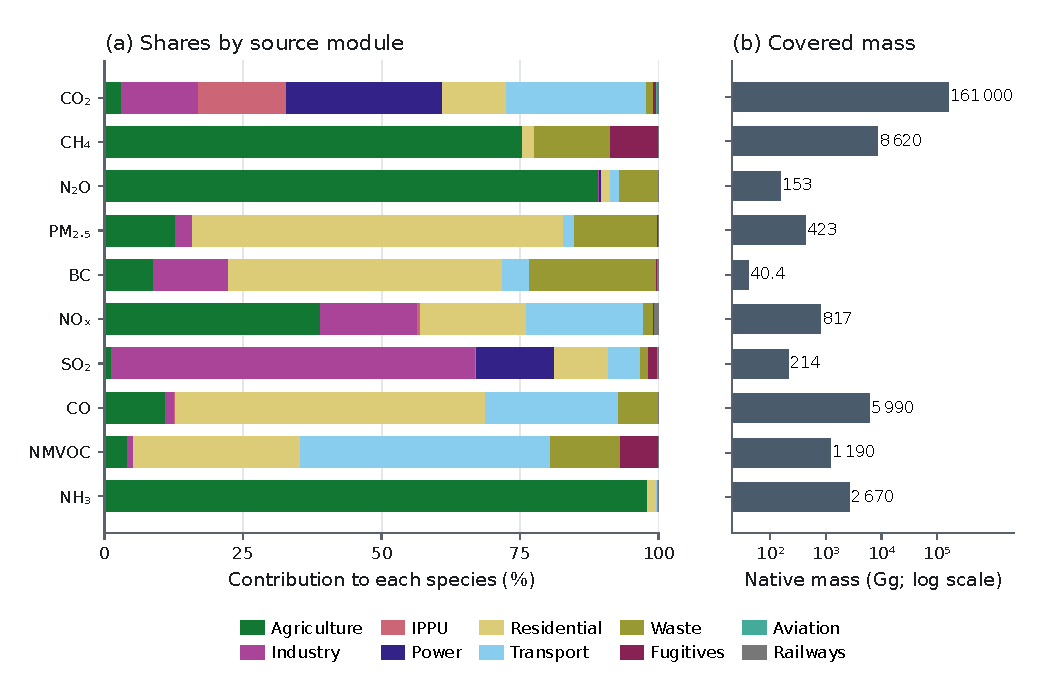
\includegraphics[width=\textwidth]{../../figures/f09_integrated_composition.pdf}
\caption{Reference-year (FY2023--24) source composition of each greenhouse gas and core air pollutant. (a) Share of each calculation module in the native mass of each species; (b) covered native mass on a logarithmic axis. Shares sum to \SI{100}{\percent} within a species; species are not additive, and BC is contained in PM$_{2.5}$. Power contributes only SO$_2$ from oil and diesel among air pollutants. Plotted values accompany the figure.}
\label{fig:composition}
\end{figure*}

\subsection{Air pollutants}
Table~\ref{tab:air_results} gives the core air pollutants. Their sources differ by species. Household fuel combustion accounts for \SI{67}{\percent} of FY2023--24 primary PM$_{2.5}$, open burning of waste for \SI{15}{\percent} and crop-residue burning for \SI{13}{\percent}. NO$_x$ has four comparable sources: agriculture (\SI{39}{\percent}, mainly fertilised and manured soils), road and other transport (\SI{21}{\percent}), households (\SI{19}{\percent}) and industry (\SI{17}{\percent}). Agriculture supplies \SI{98}{\percent} of NH$_3$, of which managed soils give \SI{66}{\percent} of the national total and manure management \SI{31}{\percent}. Industrial fuel combustion and cement kilns give \SI{66}{\percent} of SO$_2$ and power oil and diesel \SI{14}{\percent}. Households dominate CO (\SI{56}{\percent}) and road transport dominates NMVOC (\SI{45}{\percent}).

\begin{table}[t]
\caption{Core air pollutants in the reference and latest core years. Values are covered-source emissions in Gg (1~Gg = 1~kt). NO$_x$ is expressed as NO$_2$. BC is contained in PM$_{2.5}$.}
\label{tab:air_results}
\begin{tabular}{lrr}
\tophline
Species & FY2023--24 & FY2024--25 \\
\middlehline
Primary PM$_{2.5}$ & \num{\AirReferencePM} & \num{\AirLatestPM} \\
BC & \num{\AirReferenceBC} & \num{\AirLatestBC} \\
NO$_x$ & \num{\AirReferenceNOx} & \num{\AirLatestNOx} \\
SO$_2$ & \num{\AirReferenceSOtwo} & \num{\AirLatestSOtwo} \\
CO & \num{\AirReferenceCO} & \num{\AirLatestCO} \\
NMVOC & \num{\AirReferenceNMVOC} & \num{\AirLatestNMVOC} \\
NH$_3$ & \num{\AirReferenceNHthree} & \num{\AirLatestNHthree} \\
\bottomhline
\end{tabular}
\end{table}

Agriculture leads both the GHG aggregate and NH$_3$, while households lead PM$_{2.5}$ and CO and are a smaller part of the GHG aggregate. Such contrasts follow from the processes and are specific to each pair of species; they are not a general ordering of GHGs against pollutants. Emission mass by source is not a ranking of exposure or of health effects, which also depend on release height, location, timing and atmospheric chemistry.

\subsection{Trends}
The GHG aggregate changes by \SI{\PakChangeARfive}{\percent} between FY2015--16 and FY2024--25 (Fig.~\ref{fig:trends}). Within paired realisations the change is \SI{59.4}{\mega\tonne}, with a conditional 95\,\% interval of \SIrange{44.1}{79.5}{\mega\tonne} under persistent parameters. Of the \num{9} consecutive annual changes, \num{6} have intervals that exclude zero under persistent parameters and \num{4} under independently resampled annual activity errors, so year-to-year statements depend on the assumed error dependence. Over the same period primary PM$_{2.5}$ changes by \SI{\PakChangePMfine}{\percent}, NO$_x$ by \SI{\PakChangeNOx}{\percent}, NH$_3$ by \SI{\PakChangeNHthree}{\percent} and SO$_2$ by \SI{\PakChangeSOtwo}{\percent}. The provisional FY2025--26 sources are excluded from these common-core endpoints.

The trends have different evidential bases. Station fuel, product sales and crop and fertiliser statistics give observed annual activity. Livestock numbers are reconstructed on the census anchor, household fuel is interpolated or extrapolated between surveys, and management shares are fixed. The SO$_2$ series should not be read as a measured decline. Covered power, which admits oil and diesel only, changes by \SI{-228}{\giga\gram} between FY2015--16 and FY2024--25 (from \SI{233}{\giga\gram} to \SI{5.7}{\giga\gram}) as oil-fired generation falls, while coal-fired generation, which grew over the period, is outside the central product. The screened power-stack SO$_2$ the covered total leaves out was \SIrange{\PakFirstPowerOmitSOtwoLowPct}{\PakFirstPowerOmitSOtwoHighPct}{\percent} of it in FY2015--16 and is \SIrange{\PakLatestPowerOmitSOtwoLowPct}{\PakLatestPowerOmitSOtwoHighPct}{\percent} in FY2024--25, between the design-controlled and uncontrolled screening cases, almost all of it coal. The omitted primary PM$_{2.5}$ rises from at most \SI{\PakFirstPowerOmitPMfineHighPct}{\percent} to at most \SI{\PakLatestPowerOmitPMfineHighPct}{\percent} of the covered total, and the omitted NO$_x$ is \SIrange{\PakLatestPowerOmitNOxLowPct}{\PakLatestPowerOmitNOxHighPct}{\percent} of it in FY2024--25. Road transport changes by \SI{-55}{\giga\gram}, almost entirely at FY2017--18, when the central diesel sulfur content steps from \num{5000} to \num{500}~ppm on the date of the import specification; this is a policy-date assumption applied to the whole road pool, not an observation of sulfur at the pump. Industrial SO$_2$ follows the coal quantities booked to brick kilns, while cement-kiln SO$_2$ follows clinker, so a published reallocation of coal from cement and other industry to brick kilns raises SO$_2$ without any change in the coal burned. Of the \SI{\PakLatestCoalSOtwoChangeGg}{\giga\gram} increase in brick-kiln SO$_2$ from FY2023--24 to FY2024--25, \SI{\PakLatestCoalSOtwoSupplyGg}{\giga\gram} follows the physical supply balance, \SI{\PakLatestCoalSOtwoSeamGg}{\giga\gram} the seam between HDIP's power column and metered station burn, \SI{\PakLatestCoalSOtwoSplitGg}{\giga\gram} the shift of the published consumer split towards brick kilns and \SI{\PakLatestCoalSOtwoVintageGg}{\giga\gram} the choice of the later print. Without these three allocation terms national SO$_2$ would have changed by \SI{\PakLatestCoalSOtwoWithoutAllocationGg}{\giga\gram} rather than risen, and primary PM$_{2.5}$ by \SI{\PakLatestCoalPMfineWithoutAllocationGg}{\giga\gram}. For the GHG aggregate the same allocation seam is \SI{1.1}{\percent} of the change from FY2015--16 to FY2024--25 but \SI{69}{\percent} of the one-year change from FY2023--24 to FY2024--25, so single-year changes in the aggregate need the coal account beside them. A fixed spatial surface can redistribute a changing national total but does not show changing local activity.

\begin{figure*}[t]
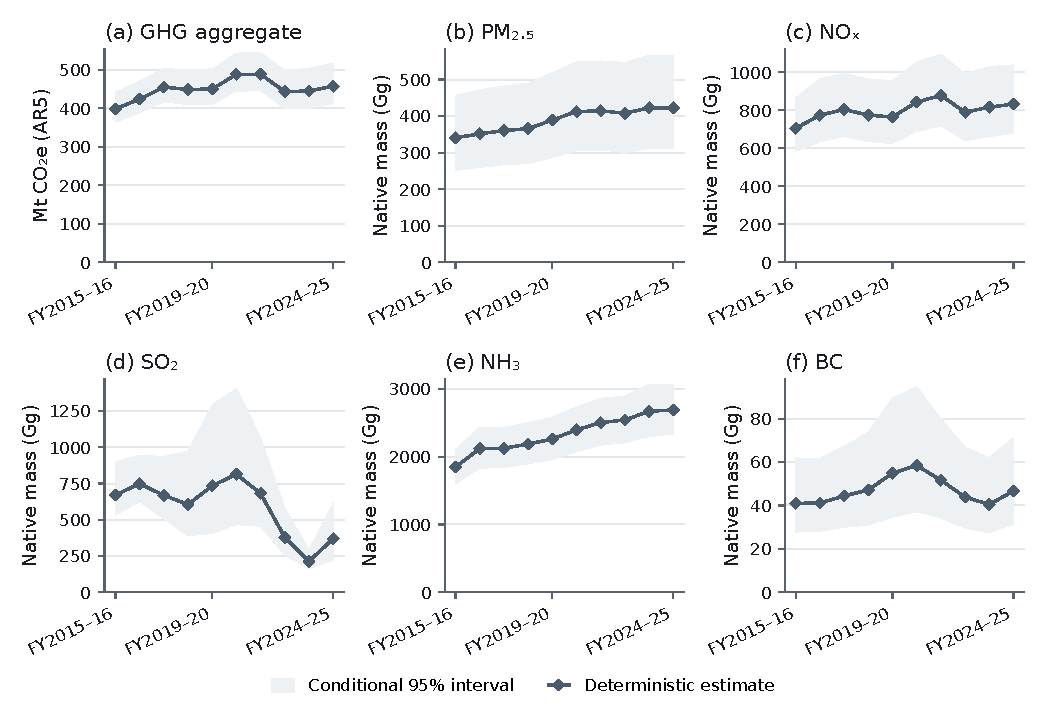
\includegraphics[width=\textwidth]{../../figures/f10_integrated_trends.pdf}
\caption{Fiscal-year series, FY2015--16 to FY2024--25, for the reference configuration: (a) GHG aggregate in Mt CO$_2$e (AR5) and (b--f) native masses of selected pollutants in Gg. Shading is the conditional 95\,\% parameter interval under persistent parameters; structural alternatives are shown in Fig.~\ref{fig:sensitivity}. The provisional FY2025--26 sources are not shown.}
\label{fig:trends}
\end{figure*}

\subsection{Uncertainty and structural sensitivity}
The FY2023--24 conditional 95\,\% interval of the GHG aggregate is \SIrange{\GHGReferenceLow}{\GHGReferenceHigh}{\mega\tonne} CO$_2$e. For the covered air sources the intervals are \SIrange{\PakRefPMfineLow}{\PakRefPMfineHigh}{\giga\gram} PM$_{2.5}$, \SIrange{\PakRefNOxLow}{\PakRefNOxHigh}{\giga\gram} NO$_x$, \SIrange{163}{293}{\giga\gram} SO$_2$ and \SIrange{\PakRefNHthreeLow}{\PakRefNHthreeHigh}{\giga\gram} NH$_3$ (Fig.~\ref{fig:sensitivity}a). Correlation diagnostics identify the leading parameters: household wood factors and biomass quantities for PM$_{2.5}$; the soil NO$_x$ fraction, followed by the cement-kiln factor, for NO$_x$; kiln-coal sulfur, brick-kiln coal and sulfur retention for SO$_2$; fertiliser volatilisation factors and poultry nitrogen for NH$_3$; and enteric and soil factors for the GHG aggregate. These diagnostics are not additive variance shares.

Structural choices move pollutants more than they move the GHG aggregate (Fig.~\ref{fig:sensitivity}b). Burning all diverted dung in households changes the GHG aggregate by about \SI{1}{\percent} but raises PM$_{2.5}$ to \SI{772}{\giga\gram}. Dated kiln-fleet cases with a long firing season raise SO$_2$ to several times the reference, because they assign more coal to kilns than the published allocation. Transferred road factors move NO$_x$, and the regional fertiliser factor moves NH$_3$. In the reference TAN configuration the all-NH$_3$ attribution diagnostic changes NO$_x$ by \SI{\PakNPartitionNOxChangeGg}{\giga\gram}, NH$_3$ by \SI{\PakNPartitionNHthreeChangeGg}{\giga\gram} and the GHG aggregate by \SI{\PakNPartitionGHGChange}{\mega\tonne} CO$_2$e. Replacing the central partition pathway by pathway with the EMEP/EEA 2023 process factors, \SI{0.04}{\kilo\gram} NO$_2$ per kilogram of fertiliser, applied manure and grazing nitrogen and \SI{0.01}{\kilo\gram} NO-N per kilogram of ammoniacal nitrogen entering solid storage \citep{EMEPEEA2023}, changes NO$_x$ by \SI{\PakRefNEmepNOxChangeGg}{\giga\gram} in the same year: the stored-manure term falls and the applied and deposited terms rise. The two nitrogen cases lie on opposite sides of the central estimate. National NO$_x$ changes by \SI{\PakChangeNOx}{\percent} from FY2015--16 to FY2024--25 centrally, by \SI{\PakChangeNOxNEmep}{\percent} with the EMEP/EEA factors and by \SI{\PakChangeNOxNPartition}{\percent} under the all-NH$_3$ diagnostic, so the partition moves the level more than the trend. None of these cases has an assigned probability, and none is a bound.

\begin{figure*}[t]
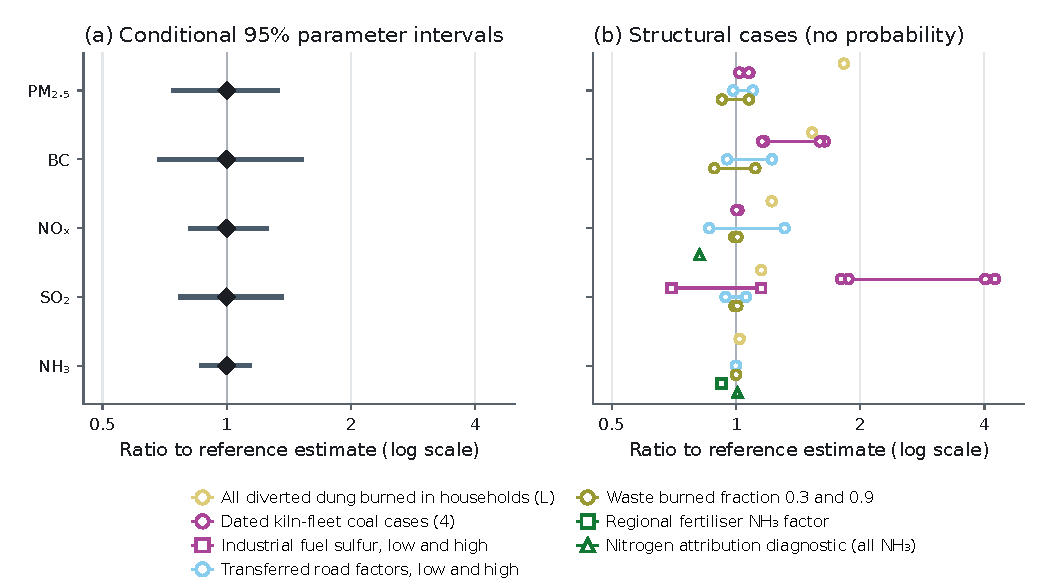
\includegraphics[width=\textwidth]{../../figures/f12_air_sensitivity.pdf}
\caption{FY2023--24 air-pollutant uncertainty for the reference configuration, as ratios to the reference estimate on a logarithmic axis. (a) Conditional 95\,\% parameter intervals. (b) Structural cases and the nitrogen attribution diagnostic, each family shown as its individual cases joined by a line; these points carry no probability and are not confidence bounds. The all-NH$_3$ diagnostic reassigns the mixed volatilisation partition and replays the nitrogen ledger.}
\label{fig:sensitivity}
\end{figure*}

\subsection{Geographic distribution}
Facility locations, household combustion, crop activity and livestock produce different spatial patterns for each species (Fig.~\ref{fig:maps}). CO$_2$ concentrates at power stations, industrial sites and cities; CH$_4$, N$_2$O and NH$_3$ follow livestock and cropland across the Indus plains; PM$_{2.5}$ follows household and burning activity. Waste is placed where it originates, which need not be where it is disposed of or burned. Unlocated facilities and activity without a supported surface remain in the unallocated account.

\begin{figure*}[t]
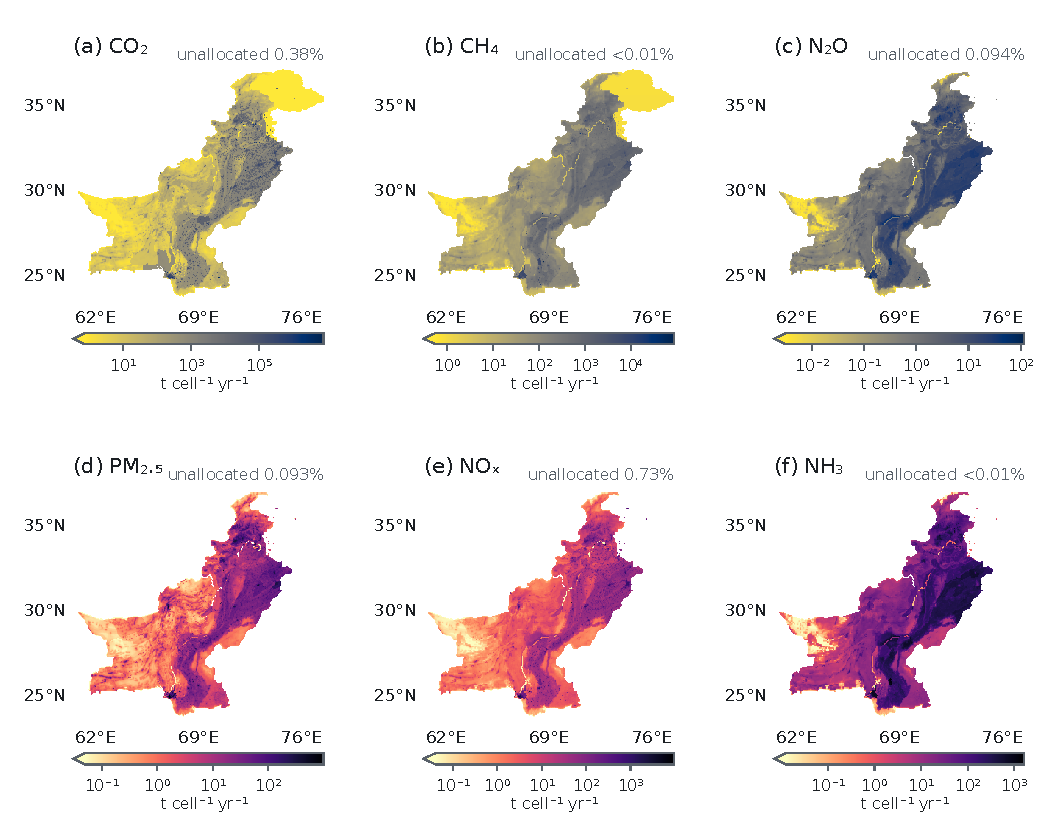
\includegraphics[width=\textwidth]{../../figures/f11_integrated_maps.pdf}
\caption{Reference-year (FY2023--24) allocated mass per \SI{0.05}{\degree} grid cell for (a--c) the greenhouse gases and (d--f) PM$_{2.5}$, NO$_x$ (as NO$_2$) and NH$_3$, in t cell$^{-1}$ yr$^{-1}$. Each panel has its own logarithmic colour scale; the lowest \SI{1}{\percent} of positive cells is shown at the lowest colour. Allocation can represent a release location, an activity origin or fuel sales, and is not an observation at grid resolution. The percentage of national mass left unallocated is printed in each panel. The outline is the statistical reporting mask and implies no position on any boundary.}
\label{fig:maps}
\end{figure*}

\section{Technical evaluation}
\label{sec:evaluation}
Evaluation separates magnitude, change, timing and location, and compares quantities only after matching period, species, mass convention, category and fuel boundary. Table~\ref{tab:validation_measured} lists what was measured directly: the source records each parser read and rejected, the closures of the monthly, gridded, district, nitrogen and coal accounts, and the rebuild comparisons of the release.

%% GENERATED by scripts/make_validation_table.py from outputs/pakemis_validation_measured.csv. Do not edit.
\begin{table*}[t]
\caption{Measured validation in the release. Records: what each check read; rejected: rows quarantined unrepaired or files that differed; closing: units that close their control, of all units; residual: the largest absolute closure residual, in the unit shown. The fifteen gridded rows that do not close are declared divergences of the three Islamabad International Airport LTO streams, which are in Islamabad Capital Territory in the provincial share table and in Attock, Punjab, on the grid. The rebuild rows compare every product file with the released one (rc68): closing counts files byte-identical to the release, the remainder being files seeded from the release and manuscripts the rebuild does not compile. The test row is the published canonical run. Sources and notes for every row are in \texttt{pakemis\_validation\_measured.csv}.}
\label{tab:validation_measured}
\small
\begin{tabular*}{\textwidth}{@{\extracolsep{\fill}}lrrrl@{}}
\tophline
Check & Records & Rejected & Closing & Largest residual \\
\middlehline
\multicolumn{5}{@{}l}{\textit{Source parsing}} \\
OCAC monthly fuel sales & 6\,055 & 2 & 36 / 36 & \num{0.1411} \% of control \\
NFDC monthly fertiliser offtake & 3\,228 & 1 & 58 / 58 & -- \\
PBS monthly minerals production & 1\,656 & 0 & 36 / 36 & -- \\
PBS manufacturing index (QIM) & 13\,536 & 9 & 1128 / 1137 & -- \\
APCMA cement dispatch & 284 & 50 & -- & -- \\
\multicolumn{5}{@{}l}{\textit{Closure}} \\
Air monthly against annual, per species & 52\,200 & -- & 70 / 70 & \num{7e-06} Gg \\
Grid against provincial shares & 1\,010 & -- & 995 / 1010 & \num{0} share \\
Districts against provinces & 6 & -- & 6 / 6 & \num{0} Mt CO$_2$e (AR5) \\
Nitrogen ledger, every year and configuration & 200 & -- & -- & \num{9.54e-07} kg N \\
Coal change decomposition & 54 & -- & -- & \num{1.64e-05} Gg / Mt CO$_2$e \\
\multicolumn{5}{@{}l}{\textit{Reproduction}} \\
rc68 clean rebuild, compiled inputs & 465 & 0 & 346 / 465 & -- \\
rc68 deposit, unpacked and built & 395 & 0 & 394 / 395 & -- \\
rc68 canonical test run & 4\,057 & 0 & 4040 / 4057 & -- \\
\bottomhline
\end{tabular*}
\end{table*}
 Many comparators share Pakistani activity statistics or factors with PakEmis, so agreement is often not independent confirmation.

Pakistan's First Biennial Transparency Report describes an inventory for FY2020--21 on AR5 warming potentials, which allows a comparison without calendar blending \citep{PakistanBTR2024}. On the categories both inventories estimate, PakEmis is \num{1.013} times the reported total. The agreement hides offsetting differences: oil and gas fugitive emissions are \num{6.91} times the reported value, enteric fermentation \num{1.22} times and domestic wastewater \num{1.79} times, while managed soils are \num{0.46} times. National agreement therefore cannot select a nitrogen formulation or a fugitive method. Comparisons with the calendar-year Common Reporting Tables, EDGAR and FAOSTAT follow the same matching and are provided with the data \citep{PakistanCRT2026,EDGAR2025,FAOSTAT2025,Tubiello2013}.

For air pollutants, industry is compared with EDGAR's fossil-only and fossil-plus-biomass fuel accounts for manufacturing combustion (IPCC 1.A.2), each with EDGAR's cement process emissions (2.A.1) added to match the integrated kiln calculation (Fig.~\ref{fig:evaluation}a) \citep{EDGARAP81}. FY2021--22 is the latest complete match because EDGAR ends in calendar 2022. Industrial SO$_2$ is \num{2.22} times EDGAR's fossil account and \num{1.93} times its fossil-plus-biomass account, while PM$_{2.5}$ is \num{0.489} and \num{0.22} times. The fuel boundary alone therefore changes a ratio by more than a factor of two before any emission factor is compared.

HTAP v3.2 is compared on matched process boundaries for every core species, with its published months summed over each July--June interval from FY2015--16 to FY2019--20 (Fig.~\ref{fig:evaluation}b). Its Pakistan road and residential sectors come from the Regional Emission inventory in ASia (REAS), extended after 2015 with EDGAR trends, and draw on international fuel and agricultural statistics that overlap PakEmis inputs \citep{HTAP2025}; agreement is therefore not independent confirmation. Road-exhaust NO$_x$ is \num{0.78} to \num{0.95} times HTAP and CO \num{0.83} to \num{1.20} times, whereas road PM$_{2.5}$ is \num{0.23} to \num{0.33} times and BC \num{0.16} to \num{0.23} times, a difference in the transferred particulate factors. Road SO$_2$ is \num{0.62} and \num{0.66} times HTAP in the first two years and \num{0.11} to \num{0.12} times from FY2017--18, when the declared diesel specification changes; HTAP has no such step. Livestock and soil NH$_3$ is \num{1.04} to \num{1.11} times HTAP in the reference configuration and \num{1.25} to \num{1.36} times in the IPCC configuration, and soil NO$_x$ \num{1.8} to \num{1.9} times in the reference. For residue burning, HTAP's mass implies emission factors \num{1.6} to \num{7.2} times those of PakEmis at the PakEmis burned dry matter, so the burned quantity is probably the main difference. Road NH$_3$, a small source, is \num{4.4} to \num{6.2} times HTAP. These comparisons locate differences in fuel boundary, sulfur dating, factor transfer and activity that a national subset of a global grid would not reveal. The CAMS-GLOB-ANT inventory requires registered access and was not used. Missing power coal pollutants in PakEmis are a coverage difference and do not indicate low plant emissions.

\begin{figure*}[t]
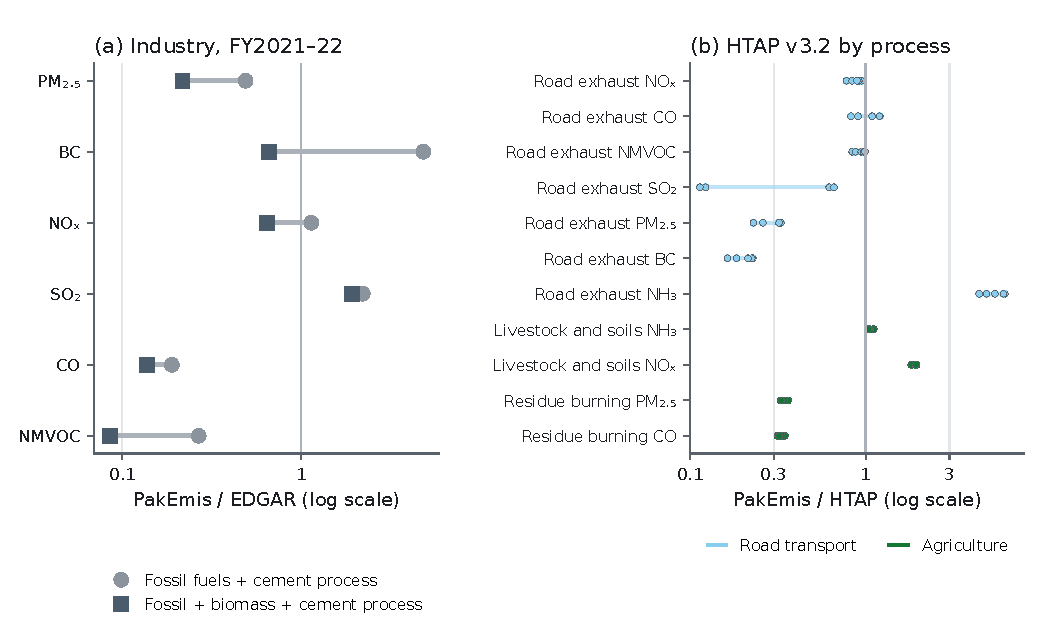
\includegraphics[width=\textwidth]{../../figures/f13_air_evaluation.pdf}
\caption{Matched-boundary air-pollutant comparisons as PakEmis/comparator ratios on logarithmic axes. (a) Industry in FY2021--22 against EDGAR v8.1 manufacturing combustion (1.A.2), fossil-only and fossil-plus-biomass, each with cement process emissions (2.A.1) added; EDGAR calendar years 2021 and 2022 are blended to the fiscal year, and other industrial processes are excluded. (b) HTAP v3.2 by process and species, FY2015--16 to FY2019--20, reference configuration; dots are the five fiscal years, summed over July--June months, and the line spans them. Shared statistics limit independence.}
\label{fig:evaluation}
\end{figure*}

Changes are evaluated against overlapping source editions and matched activity histories, with revisions kept apart from additions of new coverage. For example, the diesel customer classes of the first FY2017--18 OCAC print fall short of that edition's own printed total by an amount the following edition restores to road transport, and the inventory uses the restored road diesel. Monthly checks compare source rows and published totals with the exported records. Location checks compare facility coordinates and provincial totals, and distinguish evidence used to build an allocation from evidence held out to test it. Opposing provincial differences can cancel in a national comparison, and neither a fine grid nor agreement with a population proxy demonstrates local accuracy. Satellite columns, aerosol optical depth and fire detections can inform designed timing or location studies, but transport, chemistry and retrieval sensitivity prevent their direct use as surface-emission measurements, and no concentration--emission correlation is used as validation here.

\section{Data records and fitness for use}
\label{sec:data}
The release contains, for each of the four configurations and ten core years: native annual records by source, process and species with CO$_2$e aggregates; national, provincial and district summaries; monthly national and administrative records; annual and monthly \SI{0.05}{\degree} grids in NetCDF; conditional uncertainty levels and paired trends; structural sensitivity tables; comparison tables; and the coverage, factor, control, temporal-evidence, spatial-evidence and unallocated-mass registers. Tables are comma-separated text with typed status columns. Each record names its period, configuration, unit and estimate status, and the plotted data of every figure accompany the release.

The national totals are sums of estimated sources and should not be read as complete national emissions. The power module carries SO$_2$ only among air pollutants, so national NO$_x$, PM$_{2.5}$ and CO omit power-station coal. Little of the FY2024--25 NH$_3$ and PM$_{2.5}$ mass is placed on own-year geographic evidence: projected population and reference-year crop geography limit the interpretation of local change. Atmospheric modelling additionally needs release heights, chemical speciation and time conventions, and household emissions are gross appliance releases without an indoor-to-outdoor escape fraction. No chemical-transport simulation or health assessment is part of the release.

The primary package contains products whose redistribution terms are compatible with the Creative Commons Attribution 4.0 licence; derivatives of OpenStreetMap data under the Open Database Licence are a separate companion package. The release manifest, dependency specification, reproduction instructions and checksums identify the exact package. Reproduction from compiled activity tables is distinguished from re-extraction of primary documents.

\section{Limitations}
\label{sec:limitations}
The coal account is the largest single source of structural uncertainty for SO$_2$ and particulate matter: the published consumer allocation, the unresolved supply-minus-use quantity and the kiln-fleet cases describe different and partly incompatible coal destinations. Power-station coal pollutants are unestimated because control operation is not observed, and installed or designed controls do not establish operation. Most air-pollutant factors are transferred from European or North American measurements, and the fuel and CO$_2$ balance does not test them. Fluorinated gases, coal-mining methane and several industrial processes are unestimated, and the release gives no numerical estimate of the missing mass. Livestock history depends on a single census anchor and proxy growth, household fuel on two survey rounds and interpolation, and nitrogen fate on management shares and NO$_x$ attribution that are not measured in Pakistan. Monthly profiles for manure, evaporation, wear and several burning sources are fallbacks, and spatial patterns for population-driven and crop-driven sources often reuse reference-year surfaces.

\FloatBarrier
\conclusions
PakEmis provides annual, monthly and gridded GHG and air-pollutant records for Pakistan over July 2015--June 2025 from one set of Pakistani activity accounts. Methane from agriculture and waste is the largest part of the GHG aggregate, while household biomass combustion, agricultural nitrogen and industrial fuel combustion are the largest sources of primary PM$_{2.5}$, NH$_3$ and SO$_2$ respectively. Parameter intervals, structural configurations and unestimated sources describe different limitations and are reported separately; for several pollutants the structural cases move the estimate more than the parameter interval does. Matched comparisons show near agreement with Pakistan's own national GHG total that conceals large offsetting category differences, and pollutant ratios to global inventories that depend strongly on the fuel boundary. Better coal allocation, plant control and operating evidence, and Pakistani factor measurements would reduce the largest uncertainties more than a finer grid.

\dataavailability{PakEmis version \PakEmisRelease\ is prepared as a deposit package with product-specific licences, metadata, checksums and reproduction instructions. A persistent dataset identifier and externally accessible review deposit are pending; no DOI or review-access link is claimed here. The dataset can also be explored interactively at \url{https://emissions.hawanama.org}, a website of the Pakistan Air Quality Initiative (\url{https://pakairquality.com}). The explorer is deployed separately from the archive, and the archived release is the version of record.}
\codeavailability{The repository \url{https://github.com/PakAirQuality/pakistan-emissions-sectors} holds the source code, the verified data tables and the released products. That repository is a copy of the release without the third-party source documents, whose checksums it lists; the release manifest identifies the exact code version of the working repository and the checksums. Compiled-input and primary-source reproduction levels, documented commands and verification results accompany the deposit package.}
\authorcontribution{RA designed the inventory and its source accounting and is responsible for the scientific content.}
\competinginterests{The author declares no competing interests.}
\begin{acknowledgements}
AI coding and writing assistants (Claude, Anthropic; Codex, OpenAI) were used for code, calculations, figure production and drafting of manuscript text under the author's direction. The release records list each assisted passage, and the author is responsible for the content.
\end{acknowledgements}
%% GENERATED by scripts/make_release_cover.py from outputs/release_manifest.json.
%% Do not edit: the edit will be overwritten and CI diffs the result.
\newcommand{\ReleaseCover}{%
\begin{center}\small
\setlength{\fboxsep}{4pt}%
\fbox{\begin{minipage}{\dimexpr\linewidth-2\fboxsep-2\fboxrule\relax}\footnotesize
\textbf{Release provenance.} This document describes PakEmis under the period, configuration and source boundaries specified in its methods. The identifiers below link it to the accompanying products and source register.\\[2pt]
\begin{tabular}{@{}p{0.32\linewidth}@{\hspace{0.03\linewidth}}p{0.65\linewidth}@{}}
Release version & \texttt{1.0.0rc69} \\
Commit & \texttt{d8d874622f9a} \\
Reporting period & July 2015--June 2025 (ten fiscal years) (2015-07-01 to 2025-06-30) \\
Reference & S\_TAN (household survey; TAN nitrogen) \\
FY2023--24 total & 444.61 Mt \COe{} (AR5) under S\_TAN, the reference; 449.85 Mt under L\_TAN \\
Release manifest & \texttt{ac0ffe93ad9fcd88} (SHA-256 of \texttt{outputs/release\_manifest.json}, first 16) \\
Source manifest & \texttt{c1be6d314cfce1ea} (SHA-256 of \texttt{data/manifests/source\_manifest.csv}, first 16) \\
Data-description article & \texttt{paper\_national/} (ESSD, in preparation), same release
\end{tabular}
\end{minipage}}
\end{center}}

\ReleaseCover

\begin{thebibliography}{99}

\bibitem[Andreae(2019)]{Andreae2019}
Andreae, M. O.: Emission of trace gases and aerosols from biomass burning---an updated assessment, Atmos. Chem. Phys., 19, 8523--8546, \doi{10.5194/acp-19-8523-2019}, 2019.

\bibitem[Climate TRACE(2026)]{ClimateTRACE2026}
Climate TRACE: Climate TRACE Emissions Inventory and Data Downloads, country- and source-level records accessed through API v7 on 6 August 2026, \url{https://climatetrace.org/data}, 2026.

\bibitem[Crippa et~al.(2025)]{EDGAR2025}
Crippa, M., Guizzardi, D., Pagani, F., Banja, M., Muntean, M., Schaaf, E., Quadrelli, R., Risquez Martin, A., Taghavi-Moharamli, P., K\"oykk\"a, J., Grassi, G., Rossi, S., Melo, J., Jacome Felix Oom, D., Branco, A., Su\'arez-Moreno, M., Sedano, F., San-Miguel, J., Manca, G., Pisoni, E., and Pekar, F.: GHG emissions of all world countries---2025 report, JRC143227, Publications Office of the European Union, Luxembourg, \doi{10.2760/9816914}, 2025.

\bibitem[Crippa et~al.(2026)]{EDGARAP81}
Crippa, M., Guizzardi, D., Pagani, F., Banja, M., Muntean, M., Schaaf, E., Becker, W., Monforti Ferrario, F., Quadrelli, R., Risquez Martin, A., Grassi, G., Rossi, S., Brandao De Melo, J., Jacome Felix Oom, D., Branco, A., San-Miguel, J., and Vignati, E.: EDGAR v8.1 Global Air Pollutant Emissions, European Commission, Joint Research Centre [data set], \doi{10.2905/JRC.E1ZGQER}, 2026.

\bibitem[EEA(2023)]{EMEPEEA2023}
EEA: EMEP/EEA air pollutant emission inventory guidebook 2023, European Environment Agency, Copenhagen, \url{https://www.eea.europa.eu/publications/emep-eea-guidebook-2023}, 2023.

\bibitem[FAO(2025)]{FAOSTAT2025}
FAO: FAOSTAT: emissions totals, crops and livestock, fertilisers by nutrient, and forestry production and trade, Food and Agriculture Organization of the United Nations, Rome [data sets], \url{https://www.fao.org/faostat/}, 2025 snapshot used in the source inventory; catalogue checked 30 September 2026, 2025.

\bibitem[Government of Pakistan(2022)]{PakistanBUR2022}
Government of Pakistan: Pakistan's First Biennial Update Report to the United Nations Framework Convention on Climate Change, Ministry of Climate Change, Islamabad, \url{https://unfccc.int/documents/470405}, 2022.

\bibitem[Government of Pakistan(2024)]{PakistanBTR2024}
Government of Pakistan: Pakistan's First Biennial Transparency Report to the UNFCCC, Ministry of Climate Change and Environmental Coordination, \url{https://unfccc.int/documents/645241}, report designated 2024; UNFCCC landing page published 16 June 2025, 2024.

\bibitem[Government of Pakistan(2026)]{PakistanCRT2026}
Government of Pakistan: Pakistan: 2024 Common Reporting Table (CRT), UNFCCC submission, \url{https://unfccc.int/documents/655653}, submitted 6 February 2026, 2026.

\bibitem[Guizzardi et~al.(2025)]{HTAP2025}
Guizzardi, D., Crippa, M., Butler, T., Keating, T., Wu, R., and co-authors: The HTAP\_v3.2 emission mosaic: merging regional and global monthly emissions (2000--2020) to support air quality modelling and policies, Earth Syst. Sci. Data, 17, 5915--5950, \doi{10.5194/essd-17-5915-2025}, 2025.

\bibitem[IPCC(2006)]{IPCC2006}
IPCC: 2006 IPCC Guidelines for National Greenhouse Gas Inventories, edited by: Eggleston, H. S., Buendia, L., Miwa, K., Ngara, T., and Tanabe, K., Institute for Global Environmental Strategies, Hayama, Japan, \url{https://www.ipcc-nggip.iges.or.jp/public/2006gl/}, 2006.

\bibitem[IPCC(2013)]{IPCCAR5}
IPCC: Climate Change 2013: The Physical Science Basis, Cambridge University Press, Cambridge, \doi{10.1017/CBO9781107415324}, 2013.

\bibitem[IPCC(2019)]{IPCC2019}
IPCC: 2019 Refinement to the 2006 IPCC Guidelines for National Greenhouse Gas Inventories, edited by: Calvo Buendia, E., Tanabe, K., Kranjc, A., Baasansuren, J., Fukuda, M., Ngarize, S., Osako, A., Pyrozhenko, Y., Shermanau, P., and Federici, S., IPCC, Switzerland, \url{https://www.ipcc-nggip.iges.or.jp/public/2019rf/}, 2019.

\bibitem[IPCC(2021)]{IPCCAR6}
IPCC: Climate Change 2021: The Physical Science Basis, Cambridge University Press, Cambridge, \doi{10.1017/9781009157896}, 2021.

\bibitem[Li et~al.(2024)]{MIX2024}
Li, M., Kurokawa, J., Zhang, Q., Woo, J.-H., Morikawa, T., Chatani, S., Lu, Z., Song, Y., Geng, G., Hu, H., Kim, J., Cooper, O. R., and McDonald, B. C.: MIXv2: a long-term mosaic emission inventory for Asia (2010--2017), Atmos. Chem. Phys., 24, 3925--3952, \doi{10.5194/acp-24-3925-2024}, 2024.

\bibitem[Ministry of Finance(2026)]{MoF2026}
Ministry of Finance: Pakistan Economic Survey 2025--26, Government of Pakistan, Islamabad, agriculture and energy chapters and statistical annexes, \url{https://www.finance.gov.pk/survey/chapter_26/14_Energy.pdf}, 2026.

\bibitem[NEPRA(2025)]{NEPRA2025}
NEPRA: State of Industry Report 2025, National Electric Power Regulatory Authority, Islamabad, \url{https://nepra.org.pk/}, 2025.

\bibitem[NFDC(2025)]{NFDC2025}
NFDC: Annual Fertilizer Review 2024--25, National Fertilizer Development Centre, Government of Pakistan, \url{https://mnfsr.gov.pk/SiteImage/Misc/files/AFR2024-25.pdf}, 2025.

\bibitem[OCAC(2026)]{OCAC2026}
OCAC: Oil industry statistics: fiscal-year sectoral sales and archived editions, Oil Companies Advisory Council, Pakistan, \url{https://www.ocac.org.pk/oil-industry-statistics/archives/}, editions through July 2025--June 2026, accessed 14 October 2026.

\bibitem[PBS(2026a)]{PBSAgri2026}
PBS: Agricultural Census 2024, Pakistan Bureau of Statistics, Islamabad, report collection, \url{https://www.pbs.gov.pk/agriculture-census/}, accessed 30 September 2026, 2026a.

\bibitem[PBS(2026b)]{PBSHIES2026}
PBS: Household Integrated Economic Survey (HIES) 2024--25, Pakistan Bureau of Statistics, Islamabad, \url{https://www.pbs.gov.pk/household-integrated-economic-survey-hies-2024-25/}, accessed 30 September 2026, 2026b.

\bibitem[Runfola et~al.(2020)]{Runfola2020}
Runfola, D., Anderson, A., Baier, H., Crittenden, M., Dowker, E., Fuhrig, S., Goodman, S., Grimsley, G., Layko, R., Melville, G., Mulder, M., Oberman, R., Panganiban, J., Peck, A., Seitz, L., Shea, S., Slevin, H., Youngerman, R., and Hobbs, L.: geoBoundaries: a global database of political administrative boundaries, PLOS ONE, 15, e0231866, \doi{10.1371/journal.pone.0231866}, 2020.

\bibitem[Soulie et~al.(2024)]{CAMS2024}
Soulie, A., Granier, C., Darras, S., Zilbermann, N., Doumbia, T., Guevara, M., Jalkanen, J.-P., Keita, S., Liousse, C., Crippa, M., Guizzardi, D., Hoesly, R., and Smith, S. J.: Global anthropogenic emissions (CAMS-GLOB-ANT) for the Copernicus Atmosphere Monitoring Service simulations of air quality forecasts and reanalyses, Earth Syst. Sci. Data, 16, 2261--2279, \doi{10.5194/essd-16-2261-2024}, 2024.

\bibitem[Tubiello et~al.(2013)]{Tubiello2013}
Tubiello, F. N., Salvatore, M., Rossi, S., Ferrara, A., Fitton, N., and Smith, P.: The FAOSTAT database of greenhouse gas emissions from agriculture, Environmental Research Letters, 8, 015009, \doi{10.1088/1748-9326/8/1/015009}, 2013.

\bibitem[US EPA(1995--2025)]{AP42}
US EPA: AP-42: Compilation of Air Emissions Factors, Volume I, stationary combustion chapters and applicable revisions, United States Environmental Protection Agency, \url{https://www.epa.gov/air-emissions-factors-and-quantification/ap-42-compilation-air-emissions-factors-stationary-sources}, accessed 14 October 2026.

\end{thebibliography}
\end{document}
